\section{Methodology}

\begin{figure}[t]
  \centering 
  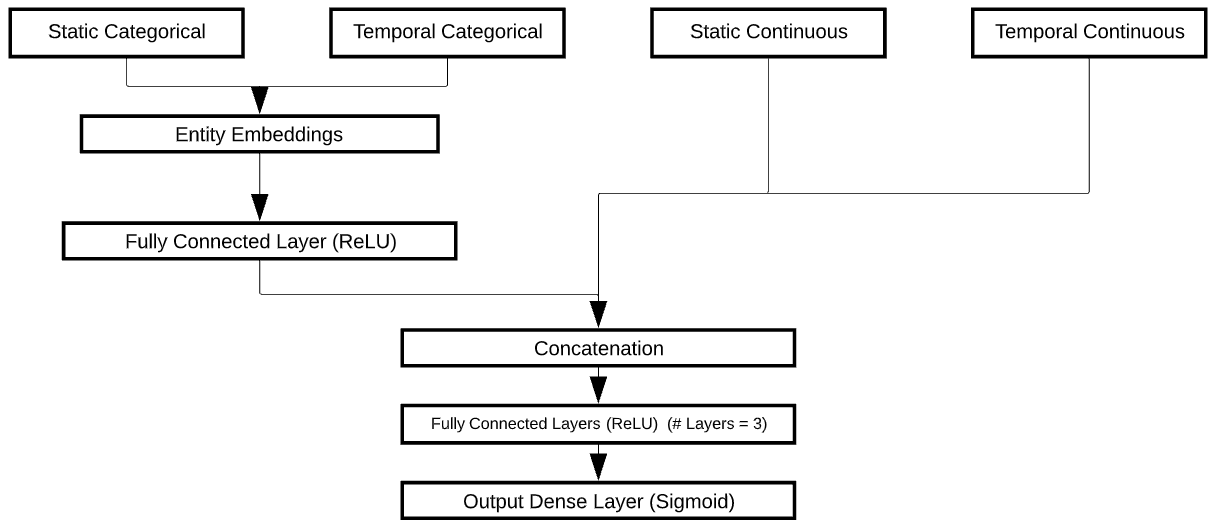
\includegraphics[width=3.3in]{img/MLP.png} 
  \caption{MLP Architecture} 
  \label{fig:MLP} 
\end{figure}

In this section, we first introduce the architecture and operation of
Software-Defined Networking (SDN). Next we give an overview of network 
reconnaissance, its utility to attackers, and the impact of successful
reconnaissance on an enterprise network's security. Finally  we discuss
how the architecture of SDN enables an adversary to perform reconnaissance 
in ways that were not feasible in traditional networks. 
In this section, we first introduce the architecture and operation of
Software-Defined Networking (SDN). Next we give an overview of network 
reconnaissance, its utility to attackers, and the impact of successful
reconnaissance on an enterprise network's security. Finally  we discuss
how the architecture of SDN enables an adversary to perform reconnaissance 
in ways that were not feasible in traditional networks. 
In this section, we first introduce the architecture and operation of
Software-Defined Networking (SDN). Next we give an overview of network 
reconnaissance, its utility to attackers, and the impact of successful
reconnaissance on an enterprise network's security. Finally  we discuss
how the architecture of SDN enables an adversary to perform reconnaissance 
in ways that were not feasible in traditional networks. 
In this section, we first introduce the architecture and operation of
Software-Defined Networking (SDN). Next we give an overview of network 
reconnaissance, its utility to attackers, and the impact of successful
reconnaissance on an enterprise network's security. Finally  we discuss
how the architecture of SDN enables an adversary to perform reconnaissance 
in ways that were not feasible in traditional networks. 
The well known Pythagorean theorem \(x^2 + y^2 = z^2\) was 
proved to be invalid for other exponents. 
Meaning the next equation has no integer solutions:
\[ x^n + y^n = z^n \]

\begin{figure}[t]
  \centering 
  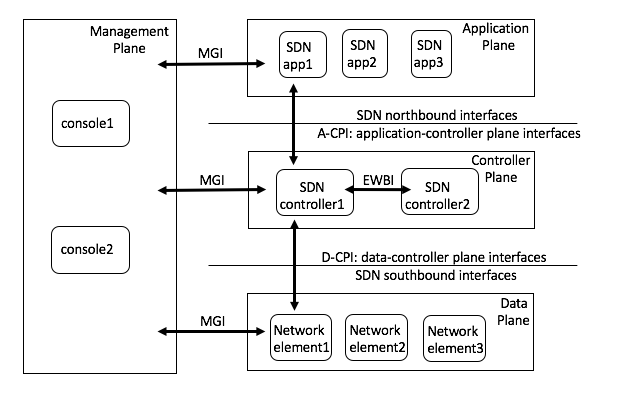
\includegraphics[width=3.3in]{img/LSTM.png} 
  \caption{LSTM Architecture} 
  \label{fig:LSTM} 
\end{figure}

In this section, we first introduce the architecture and operation of
Software-Defined Networking (SDN). Next we give an overview of network 
reconnaissance, its utility to attackers, and the impact of successful
reconnaissance on an enterprise network's security. Finally  we discuss
how the architecture of SDN enables an adversary to perform reconnaissance 
in ways that were not feasible in traditional networks. In this section, we first introduce the architecture and operation of
Software-Defined Networking (SDN). Next we give an overview of network 
reconnaissance, its utility to attackers, and the impact of successful
reconnaissance on an enterprise network's security. Finally  we discuss
how the architecture of SDN enables an adversary to perform reconnaissance 
in ways that were not feasible in traditional networks. 
In this section, we first introduce the architecture and operation of
Software-Defined Networking (SDN). Next we give an overview of network 
reconnaissance, its utility to attackers, and the impact of successful
reconnaissance on an enterprise network's security. Finally  we discuss
how the architecture of SDN enables an adversary to perform reconnaissance 
in ways that were not feasible in traditional networks. 
In this section, we first introduce the architecture and operation of
Software-Defined Networking (SDN). Next we give an overview of network 
reconnaissance, its utility to attackers, and the impact of successful
reconnaissance on an enterprise network's security. Finally  we discuss
how the architecture of SDN enables an adversary to perform reconnaissance 
in ways that were not feasible in traditional networks. In this section, we first introduce the architecture and operation of
Software-Defined Networking (SDN). Next we give an overview of network 
reconnaissance, its utility to attackers, and the impact of successful
reconnaissance on an enterprise network's security. Finally  we discuss
how the architecture of SDN enables an adversary to perform reconnaissance 
in ways that were not feasible in traditional networks. In this section, we first introduce the architecture and operation of
Software-Defined Networking (SDN). Next we give an overview of network 
reconnaissance, its utility to attackers, and the impact of successful
reconnaissance on an enterprise network's security. Finally  we discuss
how the architecture of SDN enables an adversary to perform reconnaissance 
in ways that were not feasible in traditional networks. 
In this section, we first introduce the architecture and operation of
Software-Defined Networking (SDN). Next we give an overview of network 
reconnaissance, its utility to attackers, and the impact of successful
reconnaissance on an enterprise network's security. Finally  we discuss
how the architecture of SDN enables an adversary to perform reconnaissance 
in ways that were not feasible in traditional networks. 
In this section, we first introduce the architecture and operation of
Software-Defined Networking (SDN). Next we give an overview of network 
reconnaissance, its utility to attackers, and the impact of successful
reconnaissance on an enterprise network's security. Finally  we discuss
how the architecture of SDN enables an adversary to perform reconnaissance 
in ways that were not feasible in traditional networks. 


\begin{figure}[t]
  \centering 
  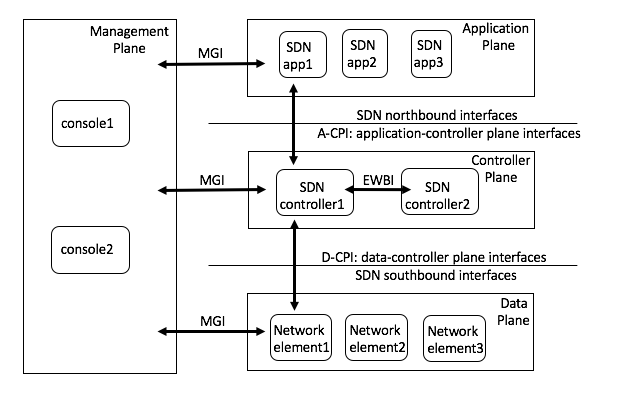
\includegraphics[width=3.3in]{img/CONV1D.png} 
  \caption{CONV1D Architecture} 
  \label{fig:CONV1D} 
\end{figure}

In this section, we first introduce the architecture and operation of
Software-Defined Networking (SDN). Next we give an overview of network 
reconnaissance, its utility to attackers, and the impact of successful
reconnaissance on an enterprise network's security. Finally  we discuss
how the architecture of SDN enables an adversary to perform reconnaissance 
in ways that were not feasible in traditional networks. 
In this section, we first introduce the architecture and operation of
Software-Defined Networking (SDN). Next we give an overview of network 
reconnaissance, its utility to attackers, and the impact of successful
reconnaissance on an enterprise network's security. Finally  we discuss
how the architecture of SDN enables an adversary to perform reconnaissance 
in ways that were not feasible in traditional networks. 
In this section, we first introduce the architecture and operation of
Software-Defined Networking (SDN). Next we give an overview of network 
reconnaissance, its utility to attackers, and the impact of successful
reconnaissance on an enterprise network's security. Finally  we discuss
how the architecture of SDN enables an adversary to perform reconnaissance 
in ways that were not feasible in traditional networks. 
In this section, we first introduce the architecture and operation of
Software-Defined Networking (SDN). Next we give an overview of network 
reconnaissance, its utility to attackers, and the impact of successful
reconnaissance on an enterprise network's security. Finally  we discuss
how the architecture of SDN enables an adversary to perform reconnaissance 
in ways that were not feasible in traditional networks. 
In this section, we first introduce the architecture and operation of
Software-Defined Networking (SDN). Next we give an overview of network 
reconnaissance, its utility to attackers, and the impact of successful
reconnaissance on an enterprise network's security. Finally  we discuss
how the architecture of SDN enables an adversary to perform reconnaissance 
in ways that were not feasible in traditional networks. In this section, we first introduce the architecture and operation of
Software-Defined Networking (SDN). Next we give an overview of network 
reconnaissance, its utility to attackers, and the impact of successful
reconnaissance on an enterprise network's security. Finally  we discuss
how the architecture of SDN enables an adversary to perform reconnaissance 
in ways that were not feasible in traditional networks. 
In this section, we first introduce the architecture and operation of
Software-Defined Networking (SDN). Next we give an overview of network 
reconnaissance, its utility to attackers, and the impact of successful
reconnaissance on an enterprise network's security. Finally  we discuss
how the architecture of SDN enables an adversary to perform reconnaissance 
in ways that were not feasible in traditional networks. 
In this section, we first introduce the architecture and operation of
Software-Defined Networking (SDN). Next we give an overview of network 
reconnaissance, its utility to attackers, and the impact of successful
reconnaissance on an enterprise network's security. Finally  we discuss
how the architecture of SDN enables an adversary to perform reconnaissance 
in ways that were not feasible in traditional networks. 


\begin{figure}[t]
  \centering 
  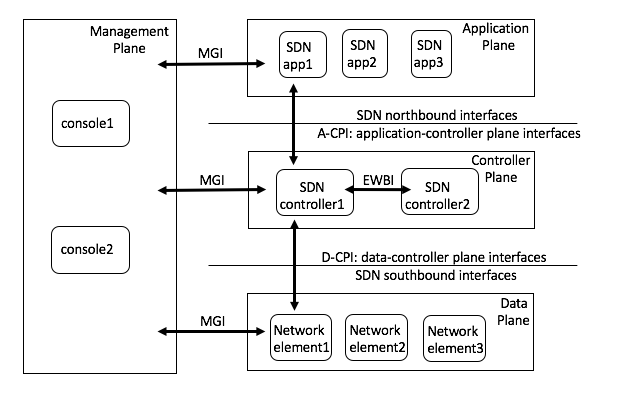
\includegraphics[width=3.3in]{img/CONV1D-LSTM.png} 
  \caption{CONV1D-LSTM Architecture} 
  \label{fig:CONV1D-LSTM} 
\end{figure}

In this section, we first introduce the architecture and operation of
Software-Defined Networking (SDN). Next we give an overview of network 
reconnaissance, its utility to attackers, and the impact of successful
reconnaissance on an enterprise network's security. Finally  we discuss
how the architecture of SDN enables an adversary to perform reconnaissance 
in ways that were not feasible in traditional networks. In this section, we first introduce the architecture and operation of
Software-Defined Networking (SDN). Next we give an overview of network 
reconnaissance, its utility to attackers, and the impact of successful
reconnaissance on an enterprise network's security. Finally  we discuss
how the architecture of SDN enables an adversary to perform reconnaissance 
in ways that were not feasible in traditional networks. 
In this section, we first introduce the architecture and operation of
Software-Defined Networking (SDN). Next we give an overview of network 
reconnaissance, its utility to attackers, and the impact of successful
reconnaissance on an enterprise network's security. Finally  we discuss
how the architecture of SDN enables an adversary to perform reconnaissance 
in ways that were not feasible in traditional networks. 
In this section, we first introduce the architecture and operation of
Software-Defined Networking (SDN). Next we give an overview of network 
reconnaissance, its utility to attackers, and the impact of successful
reconnaissance on an enterprise network's security. Finally  we discuss
how the architecture of SDN enables an adversary to perform reconnaissance 
in ways that were not feasible in traditional networks. 
In this section, we first introduce the architecture and operation of
Software-Defined Networking (SDN). Next we give an overview of network 
reconnaissance, its utility to attackers, and the impact of successful
reconnaissance on an enterprise network's security. Finally  we discuss
how the architecture of SDN enables an adversary to perform reconnaissance 
in ways that were not feasible in traditional networks. In this section, we first introduce the architecture and operation of
Software-Defined Networking (SDN). Next we give an overview of network 
reconnaissance, its utility to attackers, and the impact of successful
reconnaissance on an enterprise network's security. Finally  we discuss
how the architecture of SDN enables an adversary to perform reconnaissance 
in ways that were not feasible in traditional networks. 
In this section, we first introduce the architecture and operation of
Software-Defined Networking (SDN). Next we give an overview of network 
reconnaissance, its utility to attackers, and the impact of successful
reconnaissance on an enterprise network's security. Finally  we discuss
how the architecture of SDN enables an adversary to perform reconnaissance 
in ways that were not feasible in traditional networks. 
In this section, we first introduce the architecture and operation of
Software-Defined Networking (SDN). Next we give an overview of network 
reconnaissance, its utility to attackers, and the impact of successful
reconnaissance on an enterprise network's security. Finally  we discuss
how the architecture of SDN enables an adversary to perform reconnaissance 
in ways that were not feasible in traditional networks. 